
\begin{figure}
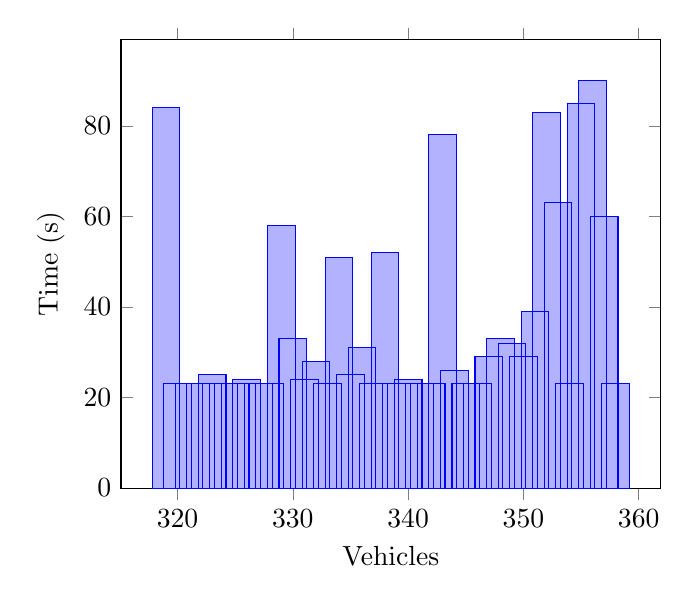
\begin{tikzpicture}
\begin{axis}[
legend style={anchor=west},
xlabel=Vehicles,
ylabel=Time (s),
ymin=0,
ybar,
]
\addplot coordinates {
(346, 23)
(347, 29)
(340, 24)
(341, 23)
(342, 23)
(343, 78)
(348, 33)
(344, 26)
(345, 23)
(339, 23)
(338, 52)
(335, 25)
(334, 51)
(337, 23)
(336, 31)
(330, 33)
(333, 23)
(332, 28)
(349, 32)
(331, 24)
(355, 85)
(322, 23)
(323, 25)
(320, 23)
(321, 23)
(326, 24)
(327, 23)
(324, 23)
(325, 23)
(328, 23)
(329, 58)
(319, 84)
(357, 60)
(356, 90)
(353, 63)
(352, 83)
(351, 39)
(350, 29)
(358, 23)
(354, 23)
};

\end{axis}
\end{tikzpicture}
\label{tik:time:100:79}
\caption{100 percent diving with GSC on route $79$}
\end{figure}
